\documentclass[11pt,a4paper]{article}

\usepackage{iftex}
\ifPDFTeX
  \usepackage[utf8]{inputenc}
  \usepackage[T1]{fontenc}
  \usepackage{lmodern}
\else
  \usepackage{fontspec}
\fi
\usepackage[english]{babel}
\usepackage[margin=2.4cm]{geometry}
\usepackage{microtype}
\usepackage{amsmath,amssymb}
\usepackage{graphicx}
\usepackage{booktabs,tabularx,array}
\usepackage{enumitem}
\usepackage{placeins}
\usepackage[hidelinks]{hyperref}
\usepackage{xurl}
\hypersetup{pdftitle={NeuroDino: Neuroevolutionary Training, Behavior Analysis and Improvement of a Small Neural Network Playing the Chrome T-Rex Game}, pdfauthor={Ahmet Şafak Yıldırım}, pdflang={en}}

\setlength{\parindent}{0pt}
\setlength{\parskip}{0.45em}
\setlist[itemize]{leftmargin=*,itemsep=0.25em,topsep=0.25em}
\setlist[enumerate]{leftmargin=*,itemsep=0.3em,topsep=0.25em}
\newcolumntype{Y}{>{\raggedright\arraybackslash}X}

\title{\textbf{NeuroDino: Neuroevolutionary Training, Behavior Analysis and Improvement of a Small Neural Network Playing the Chrome T-Rex Game}}
\author{Ahmet Şafak Yıldırım\\[0.5em]
\small Code, model and live demo: \url{https://github.com/ahm3texe/NeuroDino}}
\date{December 2025; revised October 2026}

\begin{document}
\maketitle

\begin{abstract}
In this study, a small neural network that plays the Chrome T-Rex Runner game was trained with a genetic algorithm and its behavior was measured. The agent maps 12 inputs summarizing the game state to one of the actions jump, duck and run through a fully connected 12--48--3 network (771 parameters). A population of 50 individuals, all playing the same episode in each generation, evolved for 83 generations in 6.55 hours and set a record of 547,287 points. On 200 new games, in the game loop used in training, the network reached top speed in 97.5\% of the games and completed 4 hours in 55\% of them. In the loop of the web version, where the network makes each decision with information one frame more recent, 56.5\% of the games ended before reaching top speed, while those that reached it almost never died. The geometry of the death moments and an input ablation show that the success depends on the timing of the jump to within about one frame; the network never ducks, and zeroing six of the 12 inputs does not change the outcome of any game. v2, retrained for 40 generations (57 minutes) in the web version's loop with each individual evaluated on 10 games, reached top speed in all 200 test games and completed 4 hours in 190 of them. In all 10 of v2's deaths in the test games, the dino is still in the air when it needs to jump for the next obstacle, and a fast drop by ducking in the air could have prevented every one of them. Eight neurons feeding only the duck output were added to v2, and these neurons were trained by gradient descent on frames labeled by trying both choices in the game. The resulting v3 died 3 times, against v2's 40 deaths, in 1,000 four-hour games that no model had played before. The code, the models, all evaluation games and a deterministic web version in which everyone watches the same game live are openly shared.

\textbf{Keywords:} Neuroevolution; genetic algorithms; artificial neural networks; input ablation; game agents; Chrome T-Rex.
\end{abstract}

\section{Introduction}

Video games are often used to test artificial intelligence methods because they offer controlled and reproducible dynamic environments; the success of deep reinforcement learning on Atari games is a well-known example \cite{mnih2015}. Despite their simple rules, endless runner games, which demand quick reactions and precise timing, are also well suited to studying real-time decision making.

An alternative to gradient-based reinforcement learning is neuroevolution, in which the network weights are optimized directly by evolutionary methods. Genetic algorithms and evolution strategies have been shown to compete with reinforcement learning even on deep networks \cite{such2017,salimans2017}. In problems where the reward arrives only at the end of an episode and the inputs are few, the weights of a small network can be searched for without computing gradients.

In this study, a training environment was built for the Chrome T-Rex Runner game, a small neural network was trained with a genetic algorithm, and what the trained agent does and why it dies were measured. The contributions are:
\begin{itemize}
  \item a port of the game from Chromium to Python and Pygame, and a training environment that needs no browser;
  \item the training of a network with 12 inputs and 771 parameters with a genetic algorithm, and a detailed analysis of the training process from its records;
  \item an evaluation of the trained agent on 200 new games under two different game loops, the one used in training and the one used in the demo, an examination of the causes of its deaths, and an ablation measuring which inputs it uses;
  \item a second model (v2), for which the problem found was fixed in the training setup and which was selected by measuring its robustness;
  \item an analysis that finds the cause of v2's remaining deaths, and a third model (v3) that largely removes them with added neurons, without touching v2's jumps;
  \item a deterministic web version in which everyone watches the same game at the same moment, with the network's activations shown live.
\end{itemize}

\section{Related Work}

Genetic algorithms build on Holland's work \cite{holland1975}; training the weights of feedforward networks with a genetic algorithm was first shown by Montana and Davis \cite{montana1989}. Yao presents a review covering the evolution of weights, topologies and learning rules \cite{yao1999}. While methods such as NEAT also grow the topology during evolution \cite{stanley2002}, the genetic algorithm in this study does not change the topology and evolves only the weights and biases (the neurons of v3 were added by hand). On the scale side, evolution strategies \cite{salimans2017} and a simple genetic algorithm \cite{such2017} have been shown to train networks with millions of parameters. The agent in this study, in contrast, uses 12 hand-designed features instead of pixels, and the network has only 771 (899 in v3) parameters.

To explain the behavior of the trained agent, an ablation based on removing inputs was used. This approach, which looks at how much the model's output changes when an input is removed, is treated in \cite{covert2021} as a common framework covering many explanation methods.

\section{Materials and Methods}

\subsection{Game Environment}

The TypeScript sources of the T-Rex Runner game in Chromium \cite{chromium} were ported to Python and Pygame \cite{pygame}. The rules of the game were preserved: the playfield is 600$\times$150 pixels, and the physics advances in 60 fixed steps per second, independently of real time. Speed is measured in pixels per frame, not per second; it starts at 6, increases by 0.001 every frame and reaches 13 at frame 7,000. The score is 0.025 times the distance run; top speed is reached at about 1,662 points. The obstacles are small and large cacti, coming singly or in groups, and birds, which start to appear once the speed exceeds 8.5. Birds fly at one of three heights: the bird at ${y = 50}$ passes over a running dino, the bird at ${y = 75}$ can be passed by ducking under it or by jumping over it, and the bird at ${y = 100}$ must be jumped over.

Collision detection is also as in the original game: first the outer boxes of the dino and the obstacle are compared, and if they intersect, smaller boxes specific to each shape. All boxes are axis-aligned; the original game does not compare at pixel level either. There are two differences. The training runner checks all obstacles every frame; the original game checks only the first obstacle. Also, the original game's audio cue mode doubles the gaps between obstacles. Training was done with this mode off, that is, with normal gaps, while the Gradio panel and the watch script used during development ran in this mode by default, that is, with doubled gaps.

The training runner and the watch script also process the steps of a frame in a different order. In training, in each frame the network first decides by looking at the obstacles' positions in the previous frame; then the obstacles are advanced and collisions are checked. In the watch script, the Gradio panel and the web version ported from them, the obstacles are advanced first, the network decides by looking at these new positions, and then collisions are checked. So in the watch loop the same network makes every decision seeing the obstacles one frame closer. In addition, the game's night mode is never turned on in training. Night mode is only visual, but because the stars do not draw random numbers while it is on, it changes the game's random number stream. The effect of these differences on the results is measured in Section~\ref{sec:eval}.

In headless mode, Pygame runs with a dummy display driver and the frame rate is not limited; since the physics step is still 1/60 second, the results do not depend on real time. In the version used in training, the game and the panel kept being drawn to an invisible surface in this mode as well. According to the timestamps in the training records, a total of about 8.37 million frames were processed over the 83 generations in 6.55 hours: on average about 355 frames per second, or about 5.9 times real time. In the longest generation (generation 77, about 1.69 million frames, 63 minutes) this value is about 445 frames per second. In every frame, all agents alive at that moment make a decision.

\subsection{Inputs}

The network uses 12 inputs summarizing the game state instead of raw pixels (Table~\ref{tab:inputs}). The obstacle inputs are computed for the two nearest obstacles ahead of the dino ($x_{\mathrm{obs}} > x_{\mathrm{dino}}$); if there is no obstacle, the corresponding inputs are 0. Distances are converted to times in frames so that their meaning does not change as the game speed increases. The time-to-collision input is computed as
\begin{equation}
  I_{\mathrm{Dist}} = 1 - \min\!\left(1,\ \frac{x_{\mathrm{obs}} - x_{\mathrm{dino}}}{\max(1, v)\cdot 50}\right),
  \label{eq:tti}
\end{equation}
where $x_{\mathrm{dino}}$ is the left edge of the dino and $v$ is the game's speed in pixels per frame. The input is 0 if the obstacle is 50 frames or more away and close to 1 if a collision is imminent. The gap between the two obstacles is converted in the same way, with a scale of 15 frames:
\begin{equation}
  I_{\mathrm{Gap}} = 1 - \min\!\left(1,\ \frac{x_{2} - (x_{1} + w_{1})}{\max(1, v)\cdot 15}\right).
  \label{eq:gap}
\end{equation}
While the dino is jumping, its height is given as $I_{Y} = \min\!\left(1, \max\!\left(0, (y_{\mathrm{ground}} - y)/30\right)\right)$ (in screen coordinates $y$ increases downward), and its vertical velocity as $v_y/10$, clipped to $[-1, 1]$; both are 0 while the dino is on the ground.

\begin{table}[!htbp]
  \centering
  \small
  \caption{The network's 12 inputs. Obj1 is the nearest obstacle, Obj2 the one after it.}
  \label{tab:inputs}
  \begin{tabularx}{\linewidth}{@{}r l Y l@{}}
    \toprule
    \# & Input & Definition & Range \\
    \midrule
    1 & Obj1 Dist & Time left to the obstacle, Equation~\eqref{eq:tti} & $[0, 1]$ \\
    2 & Obj1 Act & 1 if the obstacle is a bird with $y < 75$, otherwise 0 & $\{0, 1\}$ \\
    3 & Obj1 W & $\min(1,\ \text{width}/75)$ & $[0, 1]$ \\
    4--6 & Obj2 Dist, Act, W & The same, for the second obstacle & \\
    7 & Speed & $v/13$ & $[0.46, 1]$ \\
    8 & Gap & Gap between the two obstacles, Equation~\eqref{eq:gap} & $[0, 1]$ \\
    9 & DinoY & Height above the ground while jumping / 30, at most 1 & $[0, 1]$ \\
    10 & DinoVel & Vertical velocity while jumping / 10 (negative while rising) & $[-1, 1]$ \\
    11 & Air & 1 if the dino is in the air & $\{0, 1\}$ \\
    12 & Duck & 1 if the dino is ducking & $\{0, 1\}$ \\
    \bottomrule
  \end{tabularx}
\end{table}
\FloatBarrier

Three properties of this design directly affect the findings. First, although the Act input was designed to mark the bird that requires ducking, the $y < 75$ threshold selects only the bird at ${y = 50}$; since this bird passes over a running dino, it requires no action. Since the birds at ${y = 75}$ and ${y = 100}$ also have the same width, the network cannot tell these two birds apart from its inputs. Second, the dino rises about 90 pixels above the ground when jumping; since the height is divided by 30, DinoY is stuck at 1 for about 85\% of the time spent in the air. Third, an obstacle drops out of the inputs as soon as it passes the dino's left edge, even though it may still overlap the dino.

\subsection{Neural Network}

The network is a fully connected feedforward network with 12 input, 48 hidden and 3 output neurons. For an input vector $\mathbf{x}\in\mathbb{R}^{12}$,
\begin{align}
  \mathbf{h} &= \tanh(\mathbf{W}_{ih}\mathbf{x}+\mathbf{b}_{h}),\\
  \mathbf{y} &= \operatorname{softmax}(\mathbf{W}_{ho}\mathbf{h}+\mathbf{b}_{o})
\end{align}
is computed, and the agent applies the most probable action, $\operatorname*{arg\,max}(\mathbf{y})$. The network has $12\times48 + 48\times3$ weights and $48 + 3$ biases, 771 parameters in total (the 8 neurons added in v3 are described in Section~\ref{sec:v3}); the computations are done with NumPy \cite{numpy} in 64-bit floating point. Following the Glorot (Xavier) method \cite{glorot2010}, the weights are sampled from the uniform distribution
\begin{equation}
  W \sim U\!\left(-\sqrt{\frac{6}{n_{\text{in}}+n_{\text{out}}}},\ \sqrt{\frac{6}{n_{\text{in}}+n_{\text{out}}}}\right)
\end{equation}
and the biases from $U(-0.5, 0.5)$. The actions map to the game as follows: \emph{jump} starts a jump if the dino is on the ground; \emph{duck} makes the dino duck if it is on the ground and puts it into a fast drop if it is in the air; \emph{run} releases the duck and otherwise does nothing.

\subsection{Genetic Algorithm}

Instead of being trained by backpropagation, the network's parameters evolve in a population of 50 individuals. The 50 agents of a generation play the same episode together, with the same obstacle sequence; a generation ends when the last agent dies. An agent's fitness is the distance it ran until it died (score $= \lfloor 0.025 \times \text{distance} \rfloor$). The next generation is produced as follows:
\begin{itemize}
  \item \textbf{Elitism:} The two best agents are carried over unchanged.
  \item \textbf{Selection:} Each parent is the fittest of three randomly chosen agents (tournament selection \cite{goldberg1991}).
  \item \textbf{Crossover:} In uniform crossover \cite{syswerda1989}, each parameter is copied from one of the two parents with equal probability.
  \item \textbf{Mutation:} Each parameter of the child mutates with probability $R$. 8\% of the mutated parameters take a new value from $U(-1, 1)$ (shock mutation); the rest get $\mathcal{N}(0, \sigma^2)$ noise added, with $\sigma = 0.05 + 0.5R$.
\end{itemize}
The mutation rate is computed after generation $g$ ends, from the record score so far, $S_{\mathrm{record}}(g)$:
\begin{equation}
  R(g) = \min\!\left(0.25,\ \max\!\left(0.05,\ \frac{0.20\cdot 0.995^{\,g}}{1 + S_{\mathrm{record}}(g)/2000}\right)\right).
  \label{eq:rate}
\end{equation}
The rate decreases both with the generation and with the record, but does not go below 0.05. At a rate of 0.05, 5\% of the parameters mutate, and shock mutation affects only 0.4\% of the parameters.

\subsection{Training Run and Records}

The network was trained in a single run on 11 December 2025 between 12:44 and 19:17 (UTC+3), for 83 generations in 6.55 hours. Training was done on a Mac mini with Python 3.13, NumPy and Pygame; no fixed random seed was used. The best and average score of each generation and the record so far were written to a CSV file. In addition, with tensorboardX \cite{tensorboardx}, for inspection in TensorBoard \cite{abadi2015}, the game speed at the end of each generation, the mutation rate, and histograms of the weights and biases of the best individual of each generation were recorded. The recorded mutation rate was computed with a floor of 0.02 instead of the 0.05 in Equation~\eqref{eq:rate}; therefore the values 0.022 and 0.02 seen in the records from generation 42 on were not used in training. Every record-setting network was also saved.

\subsection{Visualization and Web Version}

During development, a panel was built with Gradio \cite{gradio} to inspect the decisions of the best agent. This panel was replaced by a web version that offers the same visualization publicly (Figure~\ref{fig:site}). In the web version, the Python game engine and the network were ported to TypeScript. Because a seeded random number generator is used and the exponential and hyperbolic tangent functions are computed with basic arithmetic operations only, the game is deterministic; every browser produces the same frames. The web version follows the loop order of the watch script. The page starts from a regularly updated snapshot and fast-forwards the game to the current time; this way everyone watches the same game at the same moment without any video being streamed. Every connection in the network is drawn according to the magnitude of the signal it carries at that moment (weight $\times$ activation); optionally, the distances measured by the sensors are drawn over the game.

\begin{figure}[!htbp]
  \centering
  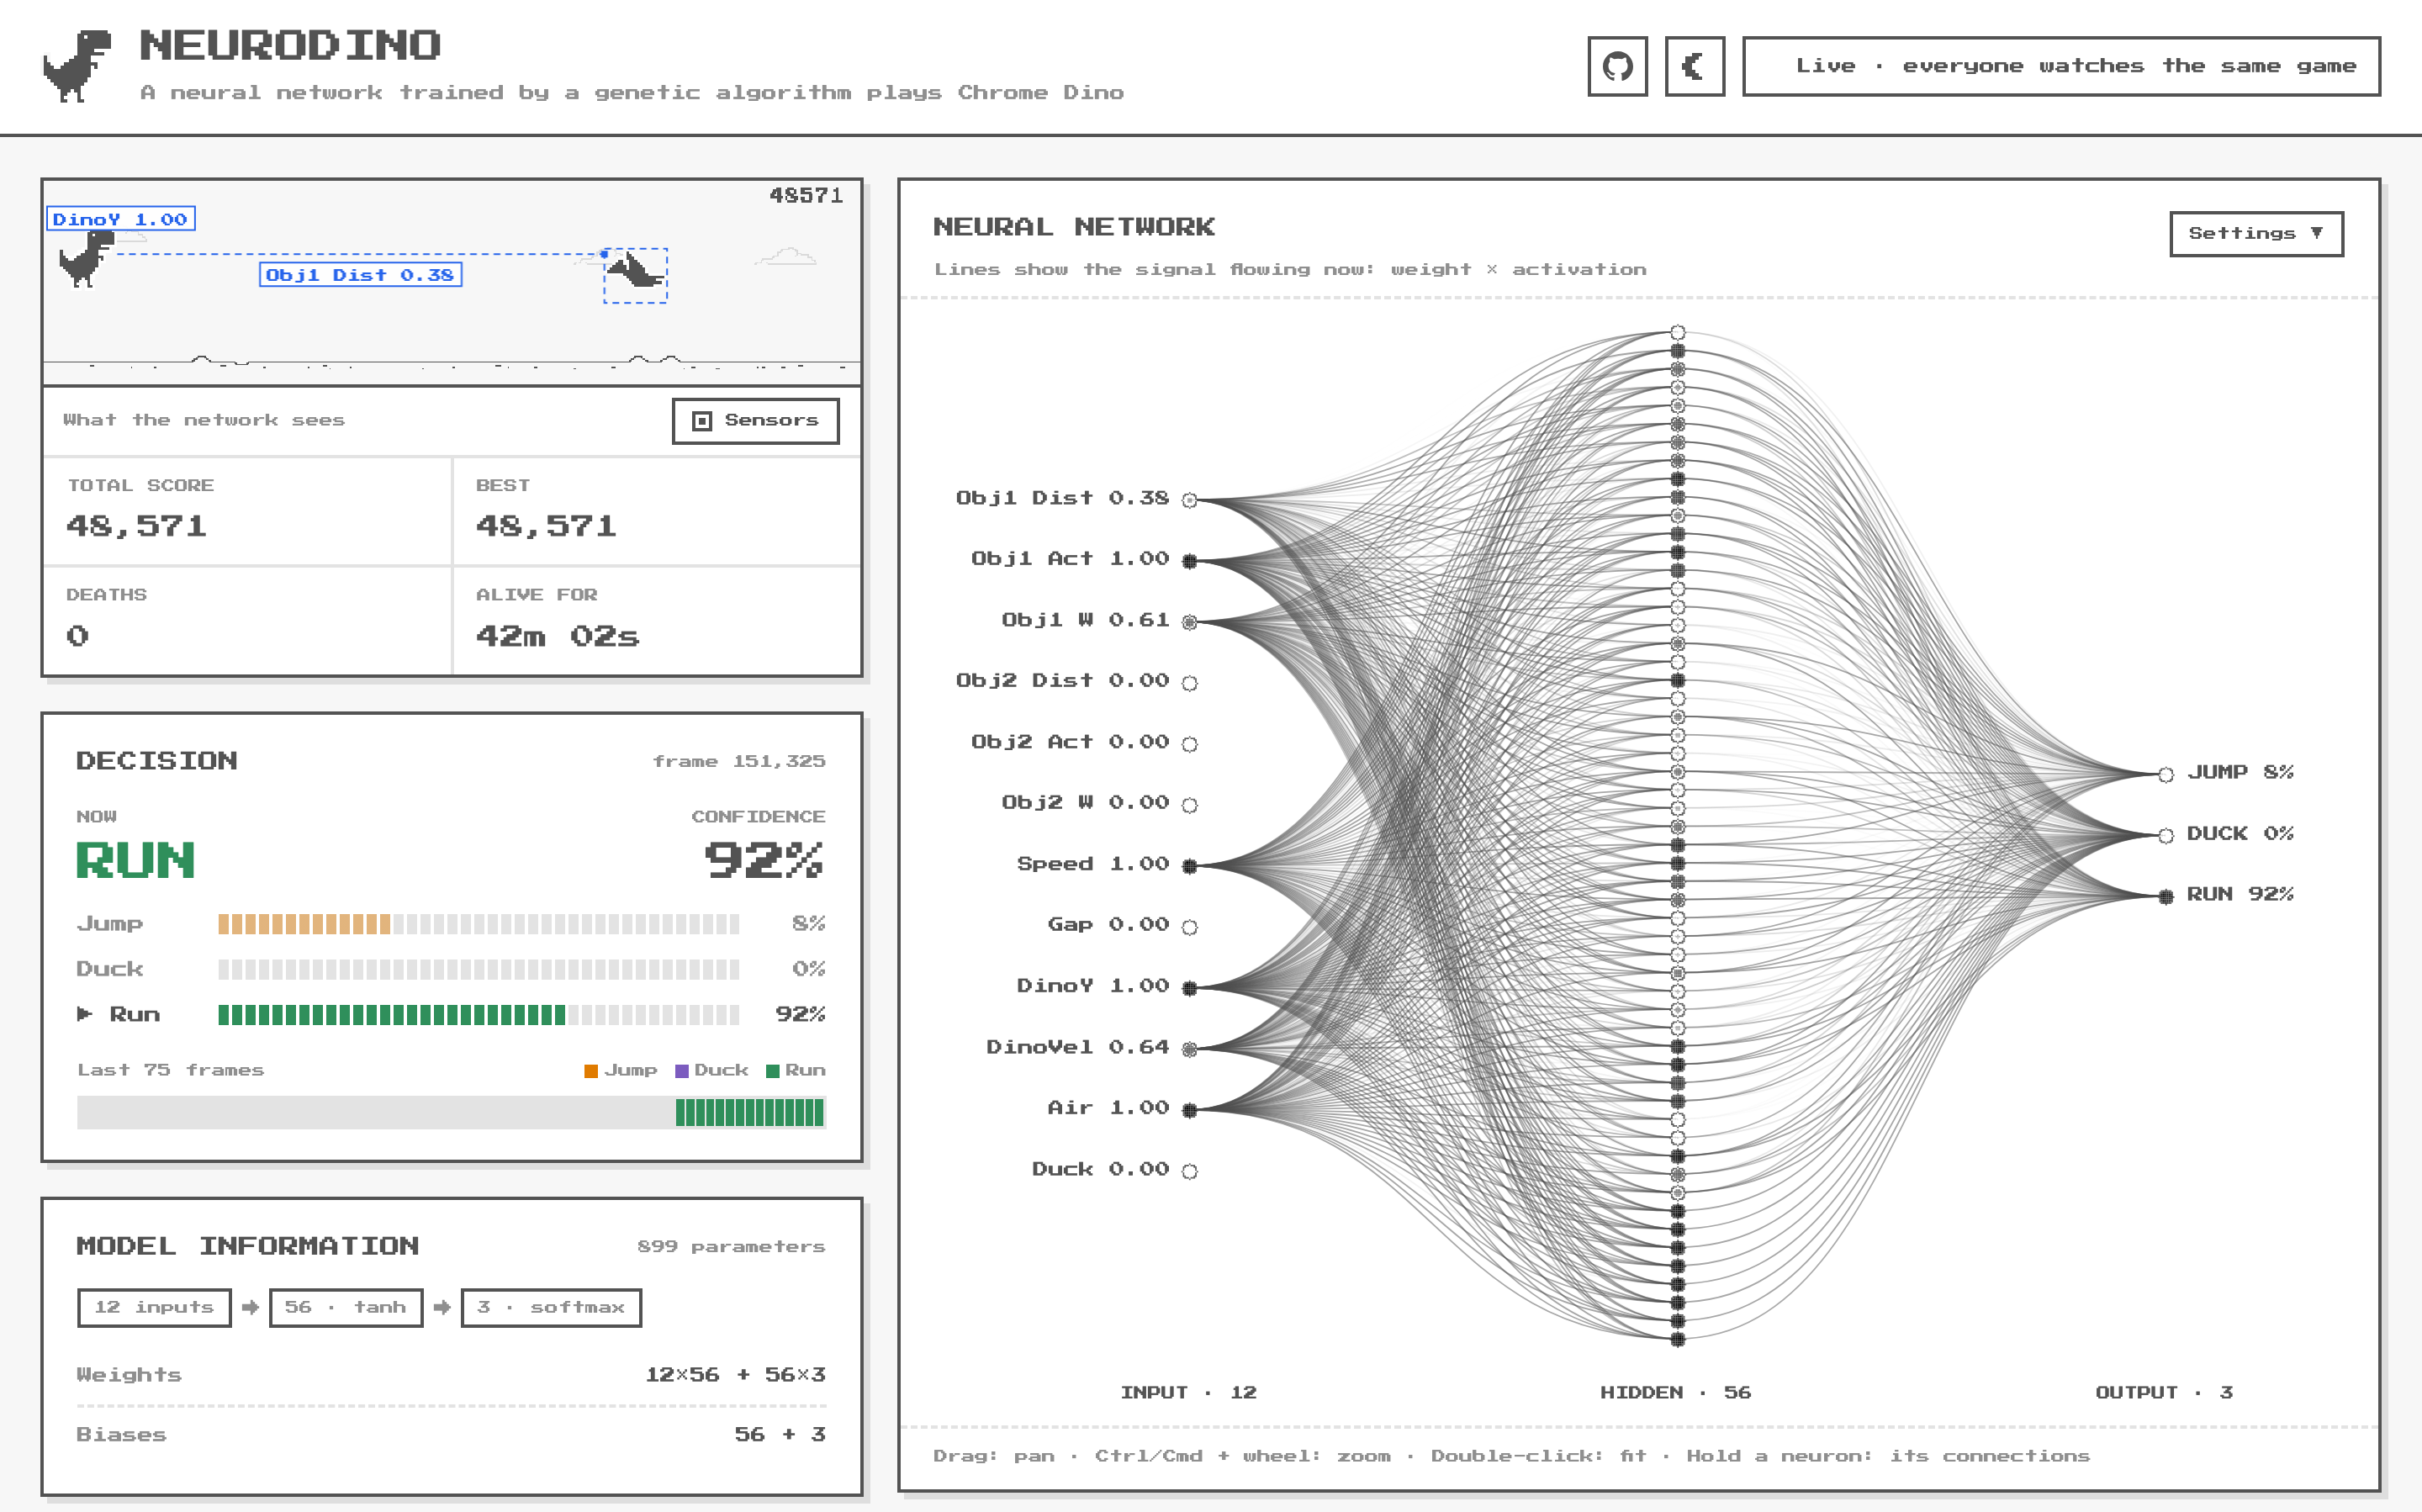
\includegraphics[width=\linewidth]{figures/website.png}
  \caption{The web version. On the left, the game, the distances measured by the sensors and the network's decision; on the right, the network: the current value of each input, the hidden layer activations and the probabilities of the three actions. The site plays v3 (56 hidden neurons). In the picture the dino is in the air and has started to descend; the next obstacle is the highest bird, which passes over a running dino (Obj1 Act $= 1$).}
  \label{fig:site}
\end{figure}
\FloatBarrier

\subsection{Evaluation Protocol}

The trained network was evaluated on new games with the TypeScript game engine of the web version. Three conditions were played with seeds from 1 to 200:
\begin{itemize}
  \item \textbf{Training conditions:} the training loop order, normal gaps and night mode off. The training order was obtained by giving the network, in each frame, the inputs at the end of the previous frame.
  \item \textbf{Website conditions:} the watch loop and normal gaps; the web version as it is today.
  \item \textbf{Demo conditions:} the watch loop and doubled gaps; the default of the Gradio panel and the watch script.
\end{itemize}
In the first two conditions each game was played until the dino died or 4 hours of game time (864,000 frames) ran out; in the third, for at most 30 minutes (108,000 frames).

The results of the TypeScript engine were verified with the Python engine. For this, the Python engine was run so that it used the same random number stream, and the single visual random number that the web version draws for the ground line was drawn on the Python side as well. The training runner (with a single agent), in the first 12,000 frames of each of 200 seeds and in five long games (up to 45,000 frames), and the watch script, in the first 20,000 frames of each of 400 games in the two gap modes and in two long games (up to 230,000 frames), died on the same frame with the same score as the TypeScript engine or survived for the same length of time.

In each game, the frame, score and speed at death; the obstacle that killed the dino (the obstacle horizontally overlapping the dino at the moment of the collision) and whether the obstacle's left edge had passed the dino's left edge at that moment; the actions chosen; the action with which each bird was passed; and the distribution of each input were recorded. The death rate at top speed was computed by dividing the number of deaths by the total game time spent at top speed, and is given with an exact 95\% confidence interval for the Poisson distribution \cite{garwood1936}. The death rates of two models were compared with a two-sided binomial test conditional on the total number of deaths of the two models.

The input ablation was done under training conditions: each input was held, in every frame, at (a) 0 or (b) its mean over all frames of the evaluation under training conditions \cite{covert2021}. Each experiment was played with the same 200 seeds for at most 30 minutes, and the games that reached top speed and the games that completed 30 minutes were counted. The code and data of the evaluation and the verification are shared in the code repository.

\section{Findings}

\subsection{Training Process}

Figure~\ref{fig:training} shows the best and average score of each generation, the record and the mutation rate. In the first 41 generations the best score did not exceed 1,247 (generation 30), and all agents died in the acceleration phase; at the end of generation 41 the speed was 8.94. In generation 42 an agent got through the acceleration phase for the first time and reached top speed, and the best score rose from 1,247 to 12,643 (about tenfold). From generation 42 on, the best agent reached top speed in all of the 42 generations. The record rose to 87,216 in generation 43, to 109,871 in generation 49 and to 547,287 in generation 77; generation 77 alone took 63 minutes.

\begin{figure}[!htbp]
  \centering
  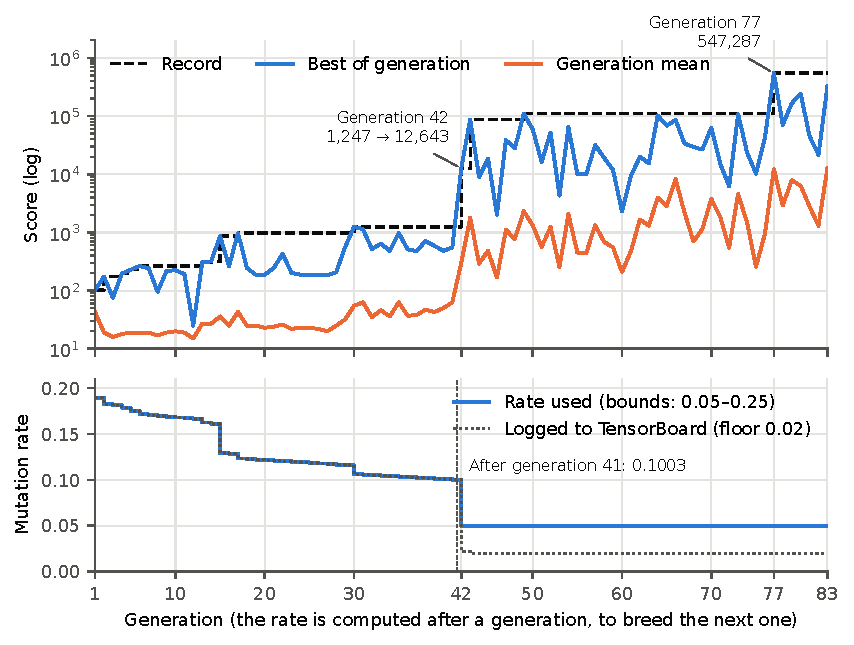
\includegraphics[width=\linewidth]{figures/training-en.pdf}
  \caption{Top: the best and average score of each generation and the record (log scale); bottom: the mutation rate. The rate is computed after a generation and breeds the next one. The rate used in training is bounded at 0.05 by Equation~\eqref{eq:rate}; the value written to TensorBoard was computed with a floor of 0.02.}
  \label{fig:training}
\end{figure}
\FloatBarrier

The relation between the mutation rate and the jump in the scores must be read carefully with respect to cause and effect. The rate that produced generation 42 is 0.1003, computed after generation 41; that is, the rate did not fall below 0.10 before the jump. The sharp drop in the plot arises when the record of generation 42 enters Equation~\eqref{eq:rate}: the formula gives 0.022, and the rate falls to its floor of 0.05. The drop is a consequence of the jump. After generation 42 the rate stayed at 0.05 until the end of training. Since there is a single run and no control experiment (for example, a run with a fixed rate), it cannot be said that the jump was caused by the adaptive mutation.

Single-episode fitness evaluation makes the scores subject to chance. The 547,287-point network was carried over unchanged to generation 78 as an elite individual, but the best score of generation 78 stayed at 70,721. So the same network scored at most 70,721 points in another episode; a large part of the record depends on the obstacle sequence of that episode. Training was stopped after generation 83 (the best score of generation 83 is 328,720).

\subsection{Weight Distributions}

Figure~\ref{fig:weights} shows the weight distributions of the record-setting networks of generations 1, 42 and 77. The weights in generation 1 lie in the uniform range of the Glorot initialization ($\pm 0.316$ for the input--hidden layer). With evolution the distributions widened: the standard deviation of the input--hidden weights rose from 0.18 to 0.33 and 0.37, and that of the hidden--output weights from 0.21 to 0.33 and 0.40; in generation 77 the input--hidden weights lie between $-1.44$ and $1.21$. These distributions show how the parameters changed; on their own they do not explain what the network learned. Since the output layer has only three biases, their histogram is not given.

\begin{figure}[!htbp]
  \centering
  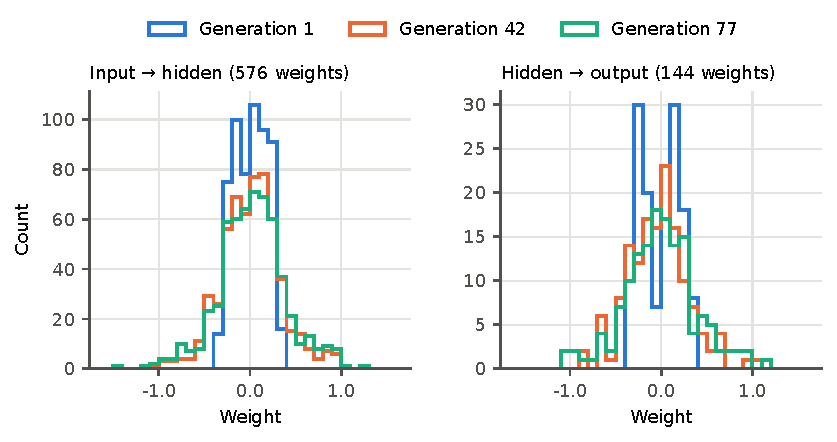
\includegraphics[width=\linewidth]{figures/weights-en.pdf}
  \caption{Weight distributions of the record-setting networks of generations 1, 42 and 77. Left: input--hidden layer; right: hidden--output layer.}
  \label{fig:weights}
\end{figure}
\FloatBarrier

\subsection{Evaluation}
\label{sec:eval}

Table~\ref{tab:conditions} and Figure~\ref{fig:eval} summarize the results under the three conditions. Under training conditions the network reached top speed in 195 of the 200 games (97.5\%); all five games that ended early ended at speed 10.8 with the bird at ${y = 75}$. At top speed, however, deaths accumulate over time: 180 of the games completed 30 minutes, 151 completed 2 hours and 110 (55\%) completed 4 hours (280,208 points). In a total of about 600 hours played at top speed there were 85 deaths, that is, about 0.14 deaths per hour (95\% confidence interval 0.11--0.18). This is consistent with the scores in training: the 547,287-point record episode lasted about 7.8 hours, while the same network's episode in generation 78 lasted at most about 1 hour (70,721 points).

\begin{table}[!htbp]
  \centering
  \small
  \caption{Number of the 200 new games that reached top speed, completed 30 minutes and completed 4 hours. Under demo conditions the games were played for at most 30 minutes.}
  \label{tab:conditions}
  \begin{tabular}{@{}l l l r r r@{}}
    \toprule
    Condition & Loop & Gaps & Top speed & 30 minutes & 4 hours \\
    \midrule
    Training & Training & Normal & 195 & 180 & 110 \\
    Website & Watch & Normal & 87 & 86 & 85 \\
    Demo & Watch & Doubled & 110 & 110 & -- \\
    \bottomrule
  \end{tabular}
\end{table}
\FloatBarrier

Under website conditions the picture is reversed. 113 of the games (56.5\%) ended before reaching top speed; these deaths cluster in four narrow speed ranges (about 7.0, 9.7--10.0, 10.5--10.8 and 12.7--12.8). Of the 87 games that reached top speed, however, only two died within 4 hours (at 23,154 and 74,243 points). Under demo conditions, since the gaps are larger, the cactus deaths around speed 7 disappeared, 90 of the games (45\%) ended early, and none of the 110 games that reached top speed died within 30 minutes.

\begin{figure}[!htbp]
  \centering
  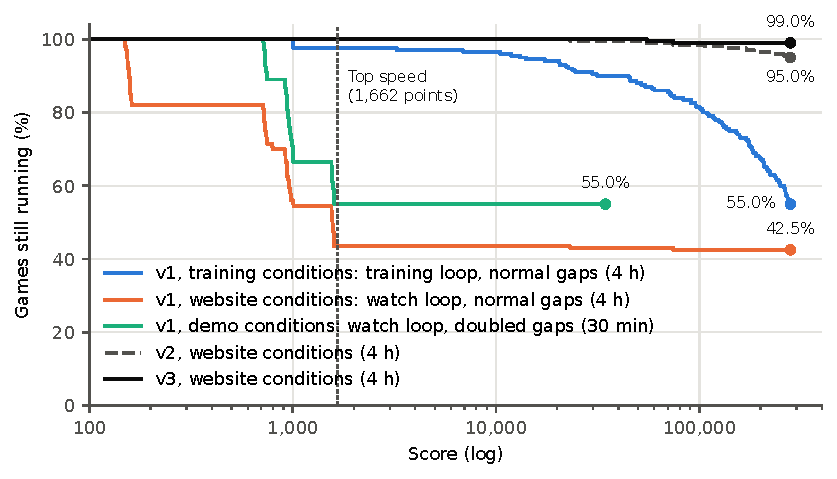
\includegraphics[width=\linewidth]{figures/evaluation-en.pdf}
  \caption{Share of the 200 new games that reach a given score: v1 under three conditions, v2 and v3 under website conditions (logarithmic horizontal axis). The vertical dashed line marks the score at which top speed is reached. Under training and website conditions the games were played for up to 4 hours, under demo conditions for up to 30 minutes. The gray dashed curve is v2, obtained by the second training in Section~\ref{sec:v2}; the black curve is v3 from Section~\ref{sec:v3}.}
  \label{fig:eval}
\end{figure}
\FloatBarrier

\subsection{Behavior Analysis}

\textbf{The network never ducks.} The \emph{duck} action was not chosen in any of the 131.1 million frames under training conditions. All but one of the 290,857 birds at ${y = 75}$ and all but three of the 290,178 birds at ${y = 100}$ were jumped over. This is a direct consequence of the input design: the Act input gives the same value for the birds at ${y = 75}$ and ${y = 100}$, and the only way to pass both of these birds is to jump. Ducking works for the bird at ${y = 75}$ and is fatal for the bird at ${y = 100}$.

\textbf{Deaths come from the timing of the jump.} The geometry at the moment of death separates two types. If the obstacle's left edge has passed the dino's left edge, the dino has landed on the obstacle, that is, it jumped early; if the obstacle is still in front of the dino, the dino jumped late or did not jump at all. Under training conditions, all 85 deaths at top speed are of the second type (72 large cacti, 13 birds at ${y = 75}$), while the five games that ended early are of the first type. Under website conditions, all 113 early deaths are of the first type. In the watch loop, since the network sees the obstacle one frame closer, the jump decision is triggered one frame early; this leads to landing on obstacles at intermediate speeds, while it largely removes the late jumps at top speed (under website conditions both deaths at top speed are also of the second type; the cause of such deaths is examined in Section~\ref{sec:v3}).

\textbf{The network uses only some of its inputs.} Table~\ref{tab:ablation} gives how often each input is nonzero under training conditions and the results of the ablation. The Gap input was not nonzero in any of the 131.1 million frames: with normal gaps the time between two obstacles never falls below 15 frames. The Duck input is also always 0, since the network never ducks. The inputs of the second obstacle are nonzero in only about 5\% of the frames.

\begin{table}[!htbp]
  \centering
  \small
  \caption{Input usage and ablation under training conditions. Nonzero: the share of all frames of the 200 games in which the input is not 0. The ablation columns give the number of the 200 games that reached top speed / completed 30 minutes; without ablation these numbers are 195 / 180. In the experiments marked *, the outcome of each of the 200 games (frame and score at death) is exactly the same as in the evaluation without ablation.}
  \label{tab:ablation}
  \begin{tabular}{@{}l r c r c@{}}
    \toprule
    Input & Nonzero & Held at 0 & Mean & Held at mean \\
    \midrule
    Obj1 Dist & 92.5\% & 0 / 0 & 0.494 & 0 / 0 \\
    Obj1 Act & 10.7\% & 0 / 0 & 0.107 & 0 / 0 \\
    Obj1 W & 92.6\% & 0 / 0 & 0.536 & 171 / 116 \\
    Obj2 Dist & 4.8\% & 195 / 180* & 0.008 & 183 / 169 \\
    Obj2 Act & 0.6\% & 194 / 179 & 0.006 & 197 / 181 \\
    Obj2 W & 4.9\% & 156 / 142 & 0.029 & 140 / 129 \\
    Speed & 100\% & 0 / 0 & 0.997 & 0 / 0 \\
    Gap & 0\% & 195 / 180* & 0 & 195 / 180* \\
    DinoY & 58.6\% & 195 / 180* & 0.537 & 0 / 0 \\
    DinoVel & 58.6\% & 195 / 180* & 0.037 & 107 / 66 \\
    Air & 58.6\% & 195 / 180* & 0.586 & 0 / 0 \\
    Duck & 0\% & 195 / 180* & 0 & 195 / 180* \\
    \bottomrule
  \end{tabular}
\end{table}
\FloatBarrier

Holding an input at 0 corresponds to removing the information it carries. When six inputs (Obj2 Dist, Gap, DinoY, DinoVel, Air and Duck) were zeroed, the outcome of none of the 200 games changed, and zeroing Obj2 Act changed the results only slightly. The ineffectiveness of DinoY, DinoVel and Air, which carry meaning in the air, is expected: while the dino is in the air, the network's decision changes something only if the fast drop (\emph{duck}) is chosen, and the network never chooses this action; while the dino is on the ground, these inputs are 0 anyway. In contrast, when the distance of the nearest obstacle, the Act input, its width or the game speed was zeroed, the agent did not reach top speed in any game. The role of Act is not ducking: with Act zeroed, 199 of the 200 deaths came from hitting the bird at ${y = 50}$; the network uses this input to adjust its jump so that it does not hit the highest bird as it approaches. Zeroing Obj2 W, in turn, worsened the result (156 instead of 195 games reached top speed).

Holding an input at its mean, on the other hand, puts the network into input combinations it did not see in training, for example by making inputs that are 0 on the ground nonzero; this column measures the network's sensitivity to small shifts rather than the information in the input. Two results directly support the timing finding. With Speed held at its mean (0.997, that is, almost top speed), all 200 games ended in the acceleration phase, and in all of them the dino landed on the obstacle: the network jumped early at every speed, as if it were at top speed, that is, it adjusts the moment of the jump to the game speed. Holding DinoVel at its mean (0.037), in turn, delayed the jump by adding a small shift to this input, which is normally 0 while the dino is on the ground: the number of games ending within 30 minutes rose from 20 to 134, and in none of these deaths did the dino land on the obstacle. A similar shift (0.036) under website conditions, on the other hand, compensated for the one-frame-early decision of the watch loop and let all 200 games reach top speed.

\section{Second Training (v2)}
\label{sec:v2}

The findings pointed to two problems: the loop order differed between training and the demo, and single-episode fitness did not reward robustness across different games. Therefore the training code was changed and a second run starting from v1 was made.

\textbf{Method.} Training was done with a new game module that includes the web version's loop (first the obstacles advance, then the network decides) and night mode. This module was verified on 200 seeds to reproduce the web version's games exactly with the same random number stream. Since the obstacles do not depend on the agents' actions, each agent in a game plays exactly the game it would have played alone. In each generation the 50 networks play the same 10 games; the games are renewed every generation, last at most 60 minutes and are played in parallel on 10 processor cores. A network's fitness is its mean score over the 10 games. Elitism, selection and crossover are as in v1; the floor of the mutation rate was lowered to 0.02 and shock mutation was removed. The initial population is v1 and 49 copies of it mutated at a rate of 0.05. All seeds are fixed; the run is exactly reproducible.

These settings were reached after a preliminary trial. In the first trial, in which the games were cut off at 30 minutes and v1's mutation settings were used, the best network found removed the early deaths but died within 30 minutes at top speed in 9\% of the games: 30-minute games did not reflect robustness at top speed in the fitness enough. In addition, the median score of the population stayed at about 50--300 points, that is, most children died at the first obstacles; when shock mutation was removed, the median score of the first generation rose from 308 to 4,090.

\textbf{Model selection.} The 40 generations took 56.8 minutes on an Apple M4. The best network of each generation was evaluated for 30 minutes on 100 validation games not used in training. The network found in generation 3 is the best in validation (mean 34,008 points, 97\% of the games completed; v1: 15,288 points, 43\%), and it remained the best of every generation up to generation 40 as an elite individual. This network was also played for 4 hours on 100 games with seeds 1001--1100; it never died early and died 3 times in 392 hours at top speed. This network was chosen as v2. The test seeds (1--200) were not used until the selection was complete.

\begin{table}[!htbp]
  \centering
  \small
  \caption{v1 and v2 on the 200 test games under website and demo conditions.}
  \label{tab:v2}
  \begin{tabular}{@{}l l r r r@{}}
    \toprule
    Model & Condition & Top speed & 30 minutes & 4 hours \\
    \midrule
    v1 & Website & 87 & 86 & 85 \\
    v2 & Website & 200 & 199 & 190 \\
    v1 & Demo & 110 & 110 & -- \\
    v2 & Demo & 200 & 200 & -- \\
    \bottomrule
  \end{tabular}
\end{table}
\FloatBarrier

\textbf{Results.} Table~\ref{tab:v2} and the gray dashed curve in Figure~\ref{fig:eval} show v2's test results. Under website conditions v2 reached top speed in all 200 games and completed 4 hours in 190 of them; v1 had died in the acceleration phase in 113 of the same games. At top speed there were 10 deaths in 775 hours, that is, about one death every 78 hours (95\% confidence interval: one every 42--162 hours); all of these deaths are of the second type, and their causes are examined in Section~\ref{sec:v3}. Under demo conditions, too, all 200 games completed 30 minutes. The results were also checked with the Python engine: there was no early death in the first 8,000 frames of 200 seeds, and the deaths in three long games happened on the same frame with the same score. Since the Act input did not change, v2 never ducks either: \emph{duck} was not chosen in any of the 168.8 million frames.

\section{Third Model (v3): Fast Drop in the Air}
\label{sec:v3}

\textbf{Problem.} v2 dies at top speed on average about once every 100 hours. All 10 deaths in the test games happened in the same situation: a single small cactus is followed by a second obstacle within 321--381 pixels (about 25--29 frames). At top speed a jump lasts 33 frames and carries the dino about 430 pixels; the dino is still in the air at the moment it needs to jump for the second obstacle. Each of these deaths was replayed from the state 60 frames before the death, and a single change was tried at each of these 60 frames: ducking for a few frames starting from that frame (a fast drop in the air), jumping at that frame, or delaying the jump by a few frames. Ducking prevented 10 of the 10 deaths; jumping earlier or later prevented none. v2 never uses this action.

\textbf{Attempt with a genetic algorithm.} First, a genetic algorithm starting from v2 and scoring the networks by their survival at these hard moments was tried. In the frames leading to the deaths, while the dino is in the air, v2's \emph{duck} output (before the softmax) is at least 1.45 (median 2.8) below the highest output. Since small mutations almost never bring it to the top, the networks' scores did not change and selection could not make progress.

\textbf{Method.} v2 was played on 4,000 games (seeds 100001--104000, 4 hours each), and the game states 45, 60, 90 and 120 frames before each of its 156 deaths at top speed were saved. The labels were obtained by actually playing both choices in the engine. From a frame in the air, the game is played twice for 150 frames: in one, the dino ducks at that frame; in the other, it does not; in both games there is no other duck until the dino lands, after which v2 plays. If only the game with the duck survives, the frame is labeled ``must duck''; if only the game without the duck survives, ``must not duck''; if both survive, it counts as ``must not duck'', since every needless duck is a new risk. In this way, every fifth frame in the air of 100 ordinary games (600001--600100) and all frames in the air after the death moments were labeled; the moments of every fifth game with a death were held out for evaluation. In the end, 4,909 ``must duck'' and 1,302,056 ``must not duck'' frames in the air and 2,260,900 ground frames from 200 ordinary games (500001--500200) were obtained.

v3 was created by adding to v2 8 hidden neurons connected only to the \emph{duck} output (12--56--3, 899 parameters). The new neurons and the duck row were trained on these labels by gradient descent using Adam \cite{kingma2015} (20,000 steps, batches of 16,384). On ground frames the target is v2's decision. v2's 48 neurons and the jump and run rows were frozen; since v2 never ducks, v3 makes the same decision as v2 in every frame in which it does not duck. After training, the bias of the duck output was lowered by 1. This value was chosen because, on the saved moments, it keeps the ducks that save the dino and reduces the needless ones: the network with the bias lowered by 1 saves 103 of the 124 death moments not used in training (74 before lowering, 77 when lowered by 2) and gets through all 4,000 tight moments that the dino normally gets through.

\textbf{Time and reproducibility.} The pipeline from v2 to v3 takes about 37 minutes on a 10-core Apple M4 with 10 parallel processes: collecting the death moments 31 minutes, sampling ordinary games and labeling 3.4 minutes, gradient descent 2.3 minutes. Evaluating a candidate on the 1,000 four-hour validation games takes 8.4 more minutes. Since all seeds are fixed, rerunning the pipeline produced the same data and a bit-identical v3.

\textbf{What did not work.} Success on the saved moments did not indicate success in long games; the candidates were compared on 1,000 four-hour validation games with seeds 300001--301000. On the same games v2 died 30 times. Training the whole network (646 deaths), adding two new inputs that give the network the time to landing (551) and neurons added without lowering the bias (125) increased the deaths despite fitting the labels well: a few decisions that changed elsewhere cost far more than they saved. Training only the duck row made little difference (23). With the added neurons, lowering the bias by 1 brought the number of deaths down to 6, and lowering it by 2 gave 9.

\begin{table}[!htbp]
  \centering
  \small
  \caption{v2 and v3 in four-hour games under website conditions. The new games (900001--901000) are games that no model had played before.}
  \label{tab:v3}
  \begin{tabular}{@{}l l r r r r@{}}
    \toprule
    Model & Games & Top speed & 4 hours & Deaths at top speed & Hours at top speed \\
    \midrule
    v2 & 200 test & 200 & 190 & 10 & 775 \\
    v3 & 200 test & 200 & 198 & 2 & 787 \\
    v2 & 1,000 new & 1,000 & 960 & 40 & 3,893 \\
    v3 & 1,000 new & 1,000 & 997 & 3 & 3,961 \\
    \bottomrule
  \end{tabular}
\end{table}
\FloatBarrier

\textbf{Results.} Since v3 was selected by looking at the validation games, it was also compared with v2 on 1,000 new games that no model had played (Table~\ref{tab:v3}). On these games v2 died 40 times, that is, about once every 100 hours (95\% confidence interval: once every 71--136 hours), while v3 died 3 times, that is, about once every 1,300 hours (95\% confidence interval: once every 450--6,400 hours). Three deaths determine v3's death rate only within a wide interval: v3 dies about 14 times less often than v2, and the 95\% confidence interval of this ratio is 4--69 times. The difference cannot be explained by chance: if the two models had the same death rate, the probability that at most 3 of the 43 deaths would fall to v3 would be very small (two-sided binomial test, $p \approx 10^{-9}$). In the test games v3 completed 4 hours in 198 of the 200 games (Figure~\ref{fig:eval}, black curve); its two deaths are in two games in which v2 also died. v3 had never played these games before the selection, but since the problem was diagnosed by looking at v2's deaths in these games, the test games should not be considered fully independent for v3; the independent comparison is the new games. Neither model has early deaths. v3 ducked in a total of 1,418 frames in the 1,000 new games, that is, rarely. The results were also checked with the Python engine: the first 20,000 frames of 200 seeds and the deaths in two long games are the same.

\section{Discussion and Limitations}

The findings show how sensitive the policy learned by a small network can be to a one-frame difference in the game loop. In training, the network learned to decide based on the obstacles' positions one frame earlier; in the watch loop the same network systematically jumps one frame early. Therefore the behavior observed in the demo and on the website does not represent the behavior under training conditions. The very long runs at top speed in the watch loop are not a general property of the network: with the same normal gaps, only two of the 87 games that reached top speed in the watch loop died within 4 hours, while in the training loop 85 of 195 games died. This is a clear example of how much evaluating a model in an environment that differs slightly from the one it was trained in can change the results.

Single-episode fitness evaluation also affects the results. Since the 50 agents of a generation play the same single episode, the scores depend on that episode's obstacle sequence and on chance; the record-setting network scoring at most 70,721 points in the next generation shows this. With about 0.14 deaths per hour at top speed, a 7.8-hour episode is also a lucky episode. In v2, evaluating each individual on 10 different games and training in the web version's loop both removed the early deaths and preserved the robustness at top speed in only 40 generations.

v3 also shows the difficulty of fixing a rare error. While a fast drop is needed about once every 100 hours, there is a chance for a wrong drop every second; so the fix must almost never be wrong. Many candidates that looked good on the saved hard moments turned out worse than v2 in long games. What worked was to keep v2's decisions completely, to teach the added neurons only the question of ``when to drop'', and to evaluate the candidates on long games.

The main limitations of the study are:
\begin{itemize}
  \item v1 consists of a single run, and no fixed random seed was used; v2 is reproducible with fixed seeds, but it is also a single run. Since there is no control experiment, no conclusion can be drawn about the effect of the adaptive mutation or of the other hyperparameters.
  \item v3 was not trained by neuroevolution alone: the added neurons learned by gradient descent from frames labeled by a search in the engine. The lowering of the duck bias and the selection of candidates were also done by hand.
  \item Since v3's death rate rests on only 3 deaths, it is known only with wide uncertainty (once every 450 to 6,400 hours); a much longer evaluation is needed for a narrower interval.
  \item The agent was not compared with other methods (NEAT, deep reinforcement learning or a rule-based agent).
  \item The input design has three flaws: the Act threshold does not mark the bird that requires ducking (v3, too, ducks only to drop fast in the air and does not know how to pass under birds), the Gap input is never nonzero with normal gaps, and DinoY saturates at 1 for about 85\% of the time spent in the air.
  \item The agent sees at most two obstacles, and the distance inputs distinguish at most 50 frames ahead; at speed 6 this is about 300 pixels, that is, half the screen.
  \item The whole evaluation was done with the TypeScript engine. That the engine gives the same results as the Python engine was verified, depending on the model and the loop, in the first 8,000 to 20,000 frames of each seed and in twelve long games, but the four-hour games were not all repeated in Python.
\end{itemize}

Future work includes redesigning the Act input to distinguish the three bird heights and having the agent also learn to duck under birds, runs repeated with several seeds, and comparison with other methods.

\section{Conclusions}

A training environment based on Python and Pygame was built for the Chrome T-Rex game, and a fixed-topology network with 771 parameters was trained with a genetic algorithm for 83 generations in 6.55 hours. The marked jump in training happened when an agent got through the acceleration phase for the first time in generation 42; the drop in the mutation rate is a consequence of this jump. Under training conditions, the record-setting network reached top speed in 97.5\% of 200 new games and, with about 0.14 deaths per hour at top speed, completed 4 hours in 55\% of the games. In the loop of the website and the demo, since the network makes every decision with information one frame more recent, the results are reversed: 56.5\% of the games end in the acceleration phase, while those that reach top speed almost never die. The network never ducks, effectively bases its decisions on the distance, type and width of the nearest obstacle and on the game speed, and its success depends on the timing of the jump to within about one frame. Repeating the training in the web version's loop, with each individual evaluated on 10 games, fixed this problem in 40 generations: v2 reached top speed in all 200 test games and completed 4 hours in 190 of them. v2's remaining deaths come from the dino not landing in time for the next obstacle after jumping over one; v3, obtained with 8 extra neurons that learned to drop fast in the air, reduced the deaths in 1,000 four-hour games that no model had played from 40 to 3, that is, about 14-fold (95\% confidence interval 4--69-fold). The deterministic web version, in which everyone watches the same game at the same moment, now plays v3 and makes it possible to observe the network's decisions live.

\section*{Code and Data}

The training and game code, the three models, the training records, the scripts that trained v3 (\texttt{training/}), and the evaluation scripts together with all games played (\texttt{evaluation/}) are at \url{https://github.com/ahm3texe/NeuroDino}. The model is published at \url{https://huggingface.co/ahm3texe/neurodino} and the live web version at \url{https://huggingface.co/spaces/ahm3texe/neurodino}. This paper is a translation of the original Turkish version, which is in the same repository (\texttt{paper/neurodino.pdf}).

\begin{thebibliography}{99}

\bibitem{mnih2015}
Mnih, V.; Kavukcuoglu, K.; Silver, D. et al. Human-level control through deep reinforcement learning. \textit{Nature}, 518(7540), 529--533, 2015.

\bibitem{such2017}
Such, F. P.; Madhavan, V.; Conti, E.; Lehman, J.; Stanley, K. O.; Clune, J. Deep Neuroevolution: Genetic Algorithms Are a Competitive Alternative for Training Deep Neural Networks for Reinforcement Learning. \textit{arXiv:1712.06567}, 2017.

\bibitem{salimans2017}
Salimans, T.; Ho, J.; Chen, X.; Sidor, S.; Sutskever, I. Evolution Strategies as a Scalable Alternative to Reinforcement Learning. \textit{arXiv:1703.03864}, 2017.

\bibitem{holland1975}
Holland, J. H. \textit{Adaptation in Natural and Artificial Systems}. University of Michigan Press, Ann Arbor, 1975.

\bibitem{montana1989}
Montana, D. J.; Davis, L. Training feedforward neural networks using genetic algorithms. In: \textit{Proceedings of the 11th International Joint Conference on Artificial Intelligence (IJCAI)}, 762--767, 1989.

\bibitem{yao1999}
Yao, X. Evolving artificial neural networks. \textit{Proceedings of the IEEE}, 87(9), 1423--1447, 1999.

\bibitem{stanley2002}
Stanley, K. O.; Miikkulainen, R. Evolving neural networks through augmenting topologies. \textit{Evolutionary Computation}, 10(2), 99--127, 2002.

\bibitem{covert2021}
Covert, I.; Lundberg, S.; Lee, S.-I. Explaining by Removing: A Unified Framework for Model Explanation. \textit{Journal of Machine Learning Research}, 22(209), 1--90, 2021.

\bibitem{chromium}
The Chromium Authors. Chrome T-Rex Runner (\texttt{dino\_game}) source code. \url{https://source.chromium.org/chromium/chromium/src/+/main:components/neterror/resources/dino_game/}. Accessed: 25 October 2026.

\bibitem{pygame}
Shinners, P. Pygame. \url{https://www.pygame.org}, 2011.

\bibitem{numpy}
Harris, C. R.; Millman, K. J.; van der Walt, S. J. et al. Array programming with NumPy. \textit{Nature}, 585(7825), 357--362, 2020.

\bibitem{glorot2010}
Glorot, X.; Bengio, Y. Understanding the difficulty of training deep feedforward neural networks. In: \textit{Proceedings of the Thirteenth International Conference on Artificial Intelligence and Statistics}, PMLR 9, 249--256, 2010.

\bibitem{goldberg1991}
Goldberg, D. E.; Deb, K. A comparative analysis of selection schemes used in genetic algorithms. In: \textit{Foundations of Genetic Algorithms}, Vol. 1, 69--93, Morgan Kaufmann, 1991.

\bibitem{syswerda1989}
Syswerda, G. Uniform crossover in genetic algorithms. In: \textit{Proceedings of the Third International Conference on Genetic Algorithms}, 2--9, Morgan Kaufmann, 1989.

\bibitem{tensorboardx}
Huang, T.-W. tensorboardX. \url{https://github.com/lanpa/tensorboardX}. Accessed: 25 October 2026.

\bibitem{abadi2015}
Abadi, M. et al. TensorFlow: Large-Scale Machine Learning on Heterogeneous Systems. Software, 2015. \url{https://www.tensorflow.org}.

\bibitem{gradio}
Abid, A.; Abdalla, A.; Abid, A.; Khan, D.; Alfozan, A.; Zou, J. Gradio: Hassle-Free Sharing and Testing of ML Models in the Wild. \textit{arXiv:1906.02569}, 2019.

\bibitem{garwood1936}
Garwood, F. Fiducial limits for the Poisson distribution. \textit{Biometrika}, 28(3/4), 437--442, 1936.

\bibitem{kingma2015}
Kingma, D. P.; Ba, J. Adam: A Method for Stochastic Optimization. In: \textit{International Conference on Learning Representations (ICLR)}, 2015.

\end{thebibliography}

\end{document}
